\section{Hardware dell'adapter board}
L'hardware utilizzato per condurre lo studio oggetto di questa tesi, consiste in due piattaforme indossabili dalle dimensioni ridotte. Ciascuna piattaforma si compone di una Adapter Board, che consiste nella scheda che monta il modulo PPG, e un microcontrollore utilizzato per l'acquisizione ed elaborazione dei segnali, in particolare è stato utilizzato STM32F4DISCOVERY, prodotto da STMicroelectronics, in entrambi i casi.
La due piattaforme si differenziano per l'Adapter Board progettata, in particolare, per il modulo PPG utilizzato che, in un caso, è il MAXM86161, e nell'altro, è il MAX86916, entrambi prodotti da Maxim Integrated.
\subsection{Adapter Board: MAXM86161}
\begin{figure}[h]
	\centering
	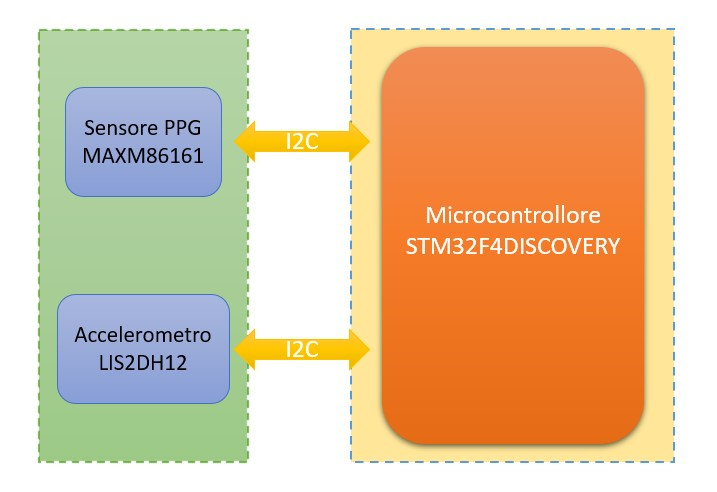
\includegraphics[width=0.8\linewidth]{ImageFiles/Hardware/diagramma_blocchi_MAXM}
	\caption{Diagramma a blocchi della piattaforma con sensore MAXM86161.}
	\label{fig:diagramma_blocchi_MAXM}
\end{figure}
L'Adapter Board è la scheda che monta il sensore PPG utilizzato per fare le acquisizioni che, vengono fatte con il microcontrollore STM32F4DISCOVERY. I due sottosistemi utilizzano il protocollo I\ap{2}C per comunicare. Come riportato in figura \Fig~\ref{fig:AssorbimentoEmolglobina}, la scheda contiene solamente il sensore PPG e un accelerometro. Grazie al numero ridotto di componenti è stato possibile ottenere una scheda dalle dimensioni molto piccole (12,4 x 4,6 mm).

\paragraph{Sensore PPG} Il sensore PPG utilizzato è il MAXM86161, prodotto da Maxim Integrated, descritto precedentemente come stato dell'arte.

\paragraph{Accelerometro} L'accelerometro utilizzato è \textbf{LIS2DH12} prodotto da STMicroelectronics. Si tratta di un circuito integrato a basso consumo e dalle piccole dimensioni (2 x 2 mm). Questo sensore viene utilizzato per migliorare la qualità delle acquisizioni fotopletismografiche quando il soggetto è in movimento, fornendo un'informazione sull'entità di quest'ultimo, e quindi del disturbo che si introduce nella misura. \todo{Parliamo anche del modello nuovo?}

\subsection{Adapter Board: MAX86916}
Questa \textit{Adapter Board} invece contiene tre circuiti integrati che sono: il sensore PPG, un regolatore di tensione (LDO) e un accelerometro.

\paragraph{Sensore PPG} Il sensore PPG utilizzato è il MAX86916, prodotto da Maxim Integrated, descritto precedentemente come stato dell'arte.

\paragraph{LDO} \todo{Parliamo dei 3 LDO che abbiamo valutato?}

\paragraph{Accelerometro} L'accelerometro utilizzato è sempre \textbf{LIS2DH12} prodotto da STMicroelectronics.

\subsection{Microcontrollore: STM32F4DISCOVERY}